\chapter{MSC: Diagramas de secuencia}
\label{ch:msc}

Según Bjorner \cite{bjorner}, los diagramas de secuencia (a partir de
ahora MSCs), \todo{AB: aquí me pones la pregunta ''de qué?''. No
  entiendo a que te refieres.} son una notación gráfica para describir
intercambios de mensajes entre entidades. Los MSCs fueron
estandarizados por primera vez por la \textit{CCITT} (conocida ahora
como la \textit{ITU-T}) en \textit{Recommendation Z.120} en 1992,
donde se especificaron sus componentes.
Se realizaron revisiones en 1996, donde se especificó la
forma en que varios MSCs (llamados \textit{basic} MSC (BMSC) pueden
ser combinados para formar un documento MSC en cual la relación entre
dichos BMSCs se describe mediante un \textit{high-level} MSC (HMSC), y
en 1999 donde se ofrecen facilidades adicionales para la
especificación de los datos que se pasan dentro de los mensajes, y se
permiten expresiones en línea.

A continuación vamos a hacer un breve resumen sobre los BMSC, que son
los diagramas que vamos a usar en \textit{Progtalk}.

\section{Basic MSCs (BMSCs)}
Un \textit{basic} MSC (a partir de ahora BMSC), esta formado por un
conjunto de instancias. Una instancia es una entidad abstracta en la
cual suceden eventos. Una instancia se nota con un cuadrado vacío, el
cual tiene una linea recta que sale verticalmente y hacia abajo desde
su base. Esta recta representa una linea temporal donde los eventos
van ocurriendo por orden cronológico de arriba hacia abajo. Los
eventos que pueden suceder entre instancias son:

\subsection*{Acciones}
Son eventos locales a una instancia. Se representan por una caja en la
línea temporal con una etiqueta en su interior. Las acciones se usan
para especificar cambios en el estado interno de la instancia,
\subsection*{Mensajes salientes} 
Representan el envío de un mensaje desde una instancia origen a otra
instancia destino.
\subsection*{Mensajes entrantes}
Representan la recepción de un mensaje. Lógicamente a cada evento de
mensaje saliente le corresponde otro evento de mensaje entrante. A
esto se le conoce como \textit{intercambio de mensajes} y se representa con una
flecha que sale de la línea temporal de la instancia origen a la
línea temporal de la instancia destino. Todo intercambio de mensajes
debe de estar etiquetado con un identificador. Podemos ver un ejemplo
de intercambio de mensajes en la figura~\ref{fig:message_exchange}

\begin{figure}
  \centering
  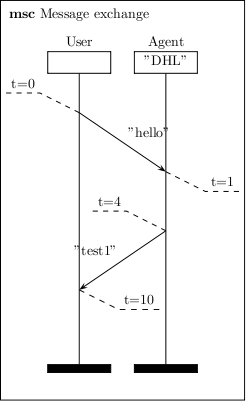
\includegraphics[scale=1]{./images/message exchange.png}
  \caption{Ejemplo de un intercambio de mensajes en un msc.}
  \label{fig:message_exchange}
\end{figure}

\subsection*{Condiciones}
Describen un estado el cual es común a un conjunto de instancias
dentro del MSC. Su fin es meramente informativo y se representan
mediante hexágonos los cuales se extienden a lo largo de las líneas de
tiempo de las instancias sobre las que la condición se aplica. El
texto de la condición debe ir en el interior del hexágono. Podemos ver
un ejemplo en la figura~\ref{fig:condition}

\begin{figure}
  \centering
  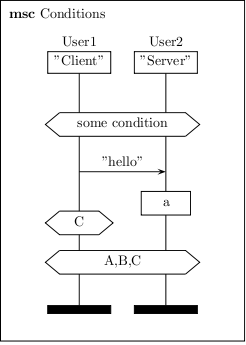
\includegraphics[scale=1]{./images/condition.png}
  \caption{Ejemplo de una condicion dentro en un msc.}
  \label{fig:condition}
\end{figure}

\subsection*{Temporizadores}
Estos eventos son locales a las instancias y como su propio nombre
indica sirven para controlar la ocurrencia temporal de los eventos
como vemos en la figura~\ref{fig:timer}. Se
nota con un reloj de arena.

\begin{figure}
  \centering
  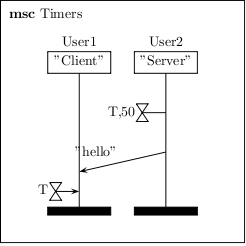
\includegraphics[scale=1]{./images/timer.png}
  \caption{Ejemplo de un temporizador dentro en un msc.}
  \label{fig:timer}
\end{figure}

\subsection*{Procesos de creación de instancias} 
Evento donde una instancia crea a otra nueva.
\subsection*{Procesos de terminación de instancias}
\todo{AB:meter ejemplos con el msc.sty}
Evento donde una instancia se termina a si misma.
\subsection*{Corregiones}
Son partes de la línea temporal de una instancia donde la premisa de
que los eventos ocurran de forma estrictamente temporal deja de ser
indispensable. Se notan con una línea discontinua y podemos ver un
ejemplo en la figura~\ref{fig:region}.

\begin{figure}
  \centering
  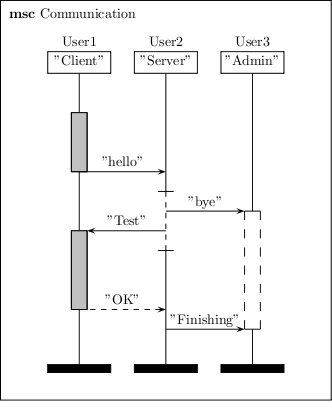
\includegraphics[scale=1]{./images/region.png}
  \caption{Ejemplo de una corregion dentro en un msc.}
  \label{fig:region}
\end{figure}

Para que un BMSC sea correcto debe cumplir las siguientes
restricciones semánticas:
\begin{itemize}
\item El nombre las instancias debe de ser único.
\item Si se especifica un interfaz para un BMSC entonces para cada
instancia en el interfaz debe haber una instancia con el mismo 
nombre y tipo en el diagrama y viceversa.
\item Todo mensaje saliente y entrante debe de referenciar una
instancia declarada en el diagrama.
\item En una instancia puede haber como mucho un mensaje de entrada
con un determinado identificador y destino, y un mensaje de salida con
un determinado identificador y origen.
\item Para cada mensaje de salida a una instancia debe de haber un 
mensaje de entrada a esa u otra instancia y viceversa.
\item Un mensaje de salida puede no ser causado por su correspondiente
mensaje de entrada directamente o via otro mensajes.     
Esta propiedad se verifica construyendo un orden parcial de los 
eventos de la comunicación y comprobando que el grafo dirigido 
obtenido de este orden parcial no contiene ciclos. Un evento
relacionado con un mensaje precede a todos los eventos relacionados
con un mensaje que lo siguen en una especificación de una instancia,
y todo mensaje de entrada es precedido por sus correspondientes 
mensajes de salida.
\item En la lista compartida de una condición solo podrá hacerse
referencia a instancias declaradas previamente.
\item Una condición compartida debe aparecer el mismo número de
veces en las instancias que la comparten.
\item En un proceso de creación de instancia solo podrá hacerse
referencia a instancias declaradas previamente.
\item No podrá haber más de un proceso de creación de instancia con
el mismo nombre de instancia.
\end{itemize}

\section{Los MSC en Progtalk}
En nuestro proyecto solo vamos a usar eventos de mensajes entrantes y
salientes. En la figura \ref{fig:fig5} vemos una representación
gráfica de un ejemplo de comunicación.

\begin{figure}
  \centering
  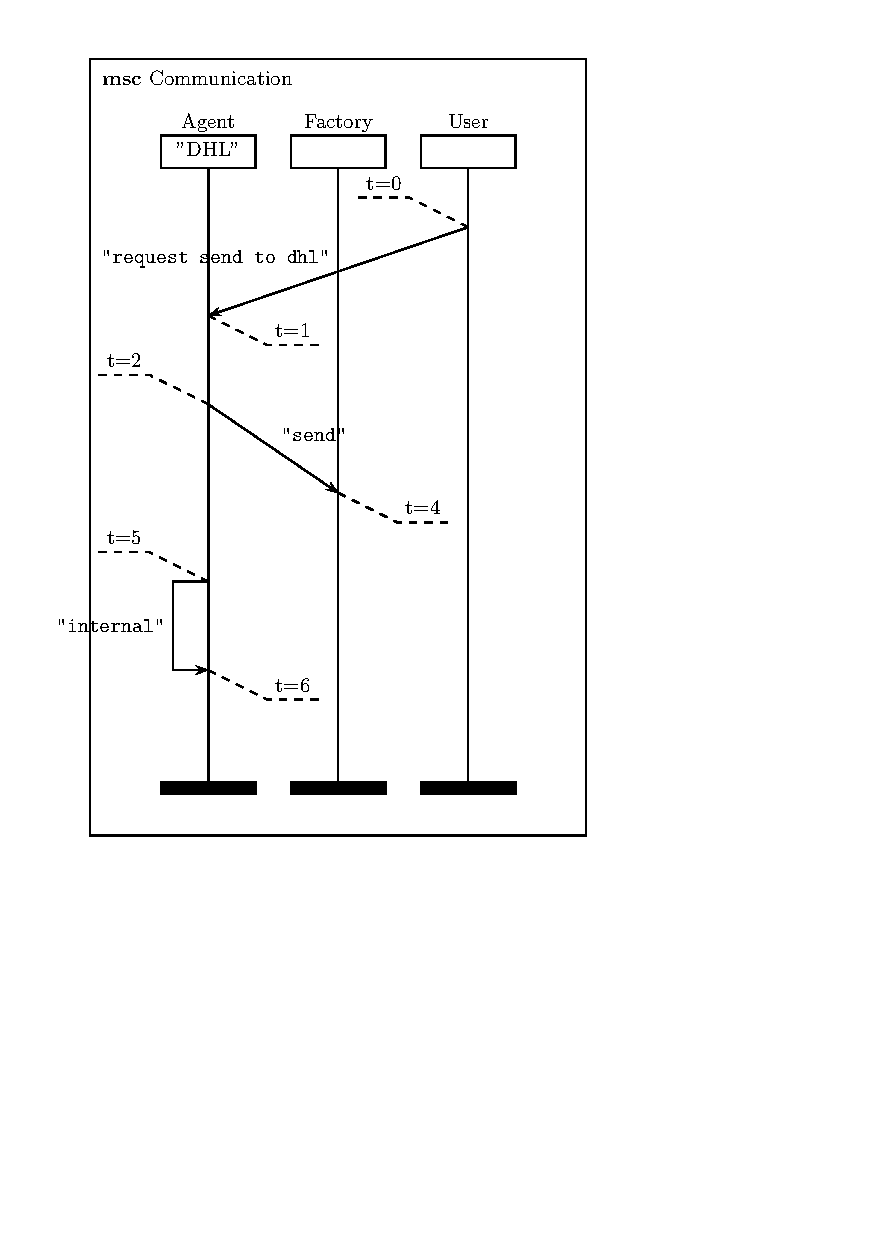
\includegraphics[scale=1]{./images/lars}
  \caption{Ejemplo de una comunicación generada con Progtalk}
  \label{fig:fig5}
\end{figure}

Para que nuestros BMSCs sean correctos deben cumplir una serie de
requisitos:
\begin{itemize}
\item Los nombres de las instancias deben de ser únicos.
\item Todos los eventos de entrada y salida deben de estar
  relacionados con una instancia ya declarada en el momento del
  evento.
\item Los identificadores de los mensajes deben de ser únicos.
\item Un tiempo de envío no pueden ser nunca mayor que su
  correspondiente tiempo de recepción (ya que no podemos mandar un
  mensaje hacia atrás en el tiempo).
\end{itemize}
\todo{AB:Aquí tras la figura 5 se nos queda una pagina en blanco que
  no viene a cuento.}

%%% Local Variables: 
%%% mode: latex
%%% TeX-master: "progtalk"
%%% TeX-PDF-mode: t
%%% ispell-local-dictionary: "castellano"
%%% End: 
